\documentclass[aspectratio=169,11pt]{beamer}

\usetheme{Boadilla}
\usecolortheme{default}
\setbeamertemplate{navigation symbols}{}
\setbeamersize{text margin left=7mm,text margin right=7mm}

\usepackage{lmodern}
\usepackage{microtype}
\usepackage{amsmath,amssymb}
\usepackage{booktabs}
\usepackage{array}
\usepackage{siunitx}
\usepackage{tikz}
\usepackage{pgfplots}
\usepackage{pgfplotstable}
\usepackage{xcolor}

\pgfplotsset{compat=1.18}
\sisetup{detect-all}
\usetikzlibrary{arrows.meta,positioning,calc,fit}

\definecolor{accentblue}{RGB}{37,84,124}
\definecolor{accentorange}{RGB}{191,102,44}
\definecolor{accentgreen}{RGB}{63,120,88}
\definecolor{lightgrayfill}{RGB}{226,231,236}

\setbeamercolor{structure}{fg=accentblue}
\setbeamercolor{frametitle}{fg=accentblue}
\setbeamercolor{title}{fg=accentblue}
\setbeamercolor{block title}{bg=accentblue!10,fg=accentblue}
\setbeamercolor{block body}{bg=accentblue!3,fg=black}

\title[Controllable NCA for Maze Navigation]{Controllable Neural Cellular Automata for\\Periodic Maze Navigation}
\subtitle[Project Summary]{Implementation Summary and Current Experimental Findings}
\author[nca-control]{nca-control project}
\date{March 30, 2026}

\begin{document}

\begin{frame}
  \titlepage
\end{frame}

\begin{frame}{Project Goal}
\begin{columns}[T,totalwidth=\textwidth]
\column{0.57\textwidth}
\begin{block}{Objective}
Learn a local NCA-style transition rule that emulates a deterministic, action-controlled grid world with exact gameplay semantics.
\end{block}
\vspace{0.4em}
\begin{itemize}
  \item periodic 2D grid with toroidal boundary conditions
  \item static blocked cells defining a solvable maze
  \item one active cell controlled by \texttt{none/up/down/left/right}
  \item exit condition with irreversible terminal lockout
  \item autonomous post-terminal fill propagation
\end{itemize}

\column{0.40\textwidth}
\centering
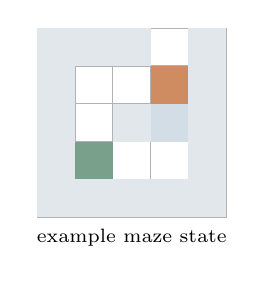
\begin{tikzpicture}[scale=0.48]
  \foreach \x in {0,...,4} {
    \foreach \y in {0,...,4} {
      \draw[gray!60] (\x,\y) rectangle ++(1,1);
    }
  }
  \foreach \x/\y in {0/4,1/4,2/4,4/4,0/3,4/3,0/2,2/2,4/2,0/1,4/1,0/0,1/0,2/0,3/0,4/0} {
    \fill[lightgrayfill] (\x,\y) rectangle ++(1,1);
  }
  \fill[accentorange!75] (3,3) rectangle ++(1,1);
  \fill[accentgreen!70] (1,1) rectangle ++(1,1);
  \fill[accentblue!20] (3,2) rectangle ++(1,1);
  \node[font=\scriptsize] at (2.5,-0.55) {example maze state};
\end{tikzpicture}

\vspace{0.3em}
\begin{tabular}{@{}ll@{}}
\textcolor{accentgreen}{$\blacksquare$} & active cell \\
\textcolor{accentorange}{$\blacksquare$} & exit / terminal fill \\
\textcolor{gray}{$\blacksquare$} & blocked cell \\
\end{tabular}
\end{columns}
\end{frame}

\begin{frame}{Task Definition}
\begin{columns}[T,totalwidth=\textwidth]
\column{0.58\textwidth}
\small
\[
\Lambda_{H,W} = \mathbb{Z}_H \times \mathbb{Z}_W
\]
\[
\mathcal{A} = \{\texttt{none}, \texttt{up}, \texttt{down}, \texttt{left}, \texttt{right}\}
\]
\[
s_t = (p_t, B, x, F_t, \tau_t)
\]
\begin{itemize}
  \item \(p_t\): active-cell position before termination
  \item \(B\): blocked cells
  \item \(x\): exit cell
  \item \(F_t\): terminal fill set
  \item \(\tau_t \in \{0,1\}\): terminal flag
\end{itemize}

\column{0.40\textwidth}
\small
\begin{block}{Reference Semantics}
\begin{enumerate}
  \item proposed move follows the input action
  \item motion wraps around the grid boundary
  \item moves into walls are cancelled
  \item reaching the exit sets the terminal flag
  \item after termination, all later inputs are ignored
  \item exit fill spreads automatically on subsequent ticks
\end{enumerate}
\end{block}
\end{columns}
\end{frame}

\begin{frame}{Implementation Approach}
\begin{columns}[T,totalwidth=\textwidth]
\column{0.51\textwidth}
\small
\begin{itemize}
  \item deterministic reference engine defines the target dynamics
  \item supervised one-step learning targets the local transition law
  \item browser visualization compares learned and reference trajectories
  \item exact rollout tests check long random action sequences
  \item inputs: active, exit-fill, blocked, and five action channels
  \item outputs: active and exit-fill with circular padding for periodicity
\end{itemize}

\column{0.47\textwidth}
\centering
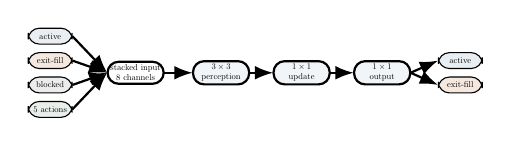
\begin{tikzpicture}[
    scale=0.31,
    transform shape,
    box/.style={draw, rounded corners, thick, align=center, minimum width=2.3cm, minimum height=0.9cm},
    smallbox/.style={draw, rounded corners, align=center, minimum width=1.8cm, minimum height=0.65cm},
    >=Latex
]
  \node[smallbox, fill=accentblue!10] (active) at (0,1.0) {active};
  \node[smallbox, fill=accentorange!15] (fill) at (0,0.0) {exit-fill};
  \node[smallbox, fill=gray!15] (blocked) at (0,-1.0) {blocked};
  \node[smallbox, fill=accentgreen!12] (action) at (0,-2.0) {5 actions};
  \node[box] (stack) at (3.5,-0.5) {stacked input\\8 channels};
  \node[box, fill=accentblue!6] (conv1) at (7.0,-0.5) {\(3\times 3\)\\perception};
  \node[box, fill=accentblue!6] (conv2) at (10.3,-0.5) {\(1\times 1\)\\update};
  \node[box, fill=accentblue!6] (head) at (13.6,-0.5) {\(1\times 1\)\\output};
  \node[smallbox, fill=accentblue!10] (preda) at (16.8,0.0) {active};
  \node[smallbox, fill=accentorange!15] (predf) at (16.8,-1.0) {exit-fill};

  \draw[->, thick] (active.east) -- (stack.west);
  \draw[->, thick] (fill.east) -- (stack.west);
  \draw[->, thick] (blocked.east) -- (stack.west);
  \draw[->, thick] (action.east) -- (stack.west);
  \draw[->, thick] (stack.east) -- (conv1.west);
  \draw[->, thick] (conv1.east) -- (conv2.west);
  \draw[->, thick] (conv2.east) -- (head.west);
  \draw[->, thick] (head.east) -- (preda.west);
  \draw[->, thick] (head.east) -- (predf.west);
\end{tikzpicture}
\end{columns}
\end{frame}

\begin{frame}{Software Stack and Evaluation Workflow}
\begin{columns}[T,totalwidth=\textwidth]
\column{0.52\textwidth}
\small
\begin{block}{Implemented Components}
\begin{itemize}
  \item deterministic grid and maze engine
  \item solvable-maze generator
  \item PyTorch and MLX training backends
  \item one-step and rollout evaluation scripts
  \item browser-based interactive verification
  \item automated testing
\end{itemize}
\end{block}

\column{0.46\textwidth}
\small
\begin{block}{Evaluation Logic}
\begin{enumerate}
  \item train on \(9\times 9\) generated mazes
  \item check exact one-step behavior
  \item test rollout exactness on larger unseen grids
  \item repeat clean retrains across seeds
\end{enumerate}
\end{block}

\vspace{0.4em}
\begin{alertblock}{Current Verified Baseline}
Selected minimal model: \texttt{12/3/1}
\end{alertblock}
\end{columns}
\end{frame}

\begin{frame}{Backend Comparison on Apple Silicon}
\begin{columns}[T,totalwidth=\textwidth]
\column{0.60\textwidth}
\begin{tikzpicture}
\begin{axis}[
    width=\linewidth,
    height=4.6cm,
    ybar,
    bar width=14pt,
    ymin=0,
    ylabel={samples/s},
    symbolic x coords={PyTorch CPU,PyTorch MPS,MLX},
    xtick=data,
    xticklabel style={rotate=20,anchor=east,font=\small},
    nodes near coords,
    every node near coord/.append style={font=\scriptsize, rotate=90, anchor=west},
    enlarge x limits=0.2,
    axis lines*=left,
]
\addplot[fill=accentblue!55] table[x=backend,y=samples_per_second,col sep=comma] {data/backend_benchmark.csv};
\end{axis}
\end{tikzpicture}

\column{0.38\textwidth}
\small
\begin{block}{Observed Result}
\begin{itemize}
  \item MLX dominates the recorded \(9\times 9\) benchmark
  \item PyTorch MPS is slower than CPU on this small workload
  \item MLX enabled stronger model sweeps and reproducibility studies
\end{itemize}
\end{block}

\begin{block}{Recorded Throughput}
\scriptsize
\begin{tabular}{@{}lr@{}}
\toprule
Backend & samples/s \\
\midrule
PyTorch CPU & 4977.51 \\
PyTorch MPS & 3082.96 \\
MLX & 40871.85 \\
\bottomrule
\end{tabular}
\end{block}
\end{columns}
\end{frame}

\begin{frame}{Minimal-Model Search}
\begin{columns}[T,totalwidth=\textwidth]
\column{0.58\textwidth}
\begin{tikzpicture}
\begin{axis}[
    width=\linewidth,
    height=4.6cm,
    ymin=0,
    ymax=1.05,
    xlabel={hidden channels},
    ylabel={accuracy / pass fraction},
    xtick=data,
    legend style={at={(0.5,-0.24)},anchor=north,legend columns=1,font=\scriptsize},
    axis lines*=left,
]
\addplot+[mark=o, thick, color=accentblue] table[x=hidden_channels,y=screen_full_state_accuracy,col sep=comma] {data/minimal_candidates.csv};
\addlegendentry{one-step screening accuracy}
\addplot+[mark=square*, thick, color=accentorange] table[x=hidden_channels,y=repro_pass_fraction,col sep=comma] {data/minimal_candidates.csv};
\addlegendentry{reproducibility pass fraction}
\end{axis}
\end{tikzpicture}

\column{0.40\textwidth}
\scriptsize
\begin{block}{Strong MLX Search Protocol}
\begin{itemize}
  \item task: \texttt{maze\_exit}
  \item grid: \(9\times 9\)
  \item mazes: \(64\)
  \item epochs: \(300\)
  \item batch size: \(128\)
  \item reproducibility seeds: \(0,1,2,3\)
\end{itemize}
\end{block}

\begin{block}{Key Finding}
\begin{itemize}
  \item \(9/3/1\): not reproducible
  \item \(10/3/1\): not exact
  \item \(11/3/1\): not reproducible
  \item \(12/3/1\): smallest exact and reproducible model found
\end{itemize}
\end{block}
\end{columns}
\end{frame}

\begin{frame}{Verification and Generalization}
\begin{columns}[T,totalwidth=\textwidth]
\column{0.58\textwidth}
\begin{block}{Fresh Post-Maintenance Checks}
\small
\begin{tabular}{@{}lcc@{}}
\toprule
Evaluation & Setting & Result \\
\midrule
One-step & \(9\times 9\) & \(1.0\) \\
Rollout & \(50\times 50\) & \(1.0\) \\
Rollout & \(100\times 100\) & \(1.0\) \\
Rollout & \(200\times 200\) & \(1.0\) \\
\bottomrule
\end{tabular}
\end{block}

\begin{block}{Interpretation}
\small
\begin{itemize}
  \item learned behavior is consistent with a shared local transition rule
  \item exactness transfers beyond the \(9\times 9\) training grid
\end{itemize}
\end{block}

\column{0.38\textwidth}
\begin{alertblock}{Large-Grid Result}
\small
The selected model remained exact on recorded rollout checks up to \(200\times 200\).
\end{alertblock}
\end{columns}
\end{frame}

\begin{frame}{Reproducibility Limits}
\begin{columns}[T,totalwidth=\textwidth]
\column{0.48\textwidth}
\small
\begin{block}{What Is Verified}
\begin{itemize}
  \item \(12/3/1\) was exact on reproducibility seeds \(0,1,2,3\)
  \item a fresh post-maintenance seed-\(0\) rerun stayed exact
  \item the same checkpoint generalized to \(50\times 50\), \(100\times 100\), and \(200\times 200\)
\end{itemize}
\end{block}

\column{0.48\textwidth}
\small
\begin{alertblock}{What Is Not Claimed}
\begin{itemize}
  \item the model is not presented as universally seed-invariant
  \item an exploratory fresh seed-\(4\) MLX run plateaued at higher loss
  \item reproducibility should therefore be described as strong on the tested seed set
\end{itemize}
\end{alertblock}
\end{columns}
\end{frame}

\begin{frame}{Conclusions}
\begin{block}{Main Findings}
\begin{itemize}
  \item controllable NCA-style local rules can emulate exact maze navigation with walls, periodic boundaries, terminal lockout, and autonomous fill dynamics
  \item the project now includes deterministic reference dynamics, automated verification, interactive visualization, and dual PyTorch/MLX backends
  \item MLX is the preferred Apple Silicon backend for this workload
  \item the current smallest exact and reproducible architecture is \(12/3/1\)
\end{itemize}
\end{block}

\begin{block}{Open Direction}
The main deferred research question is whether patch-local supervision can preserve exactness and reproducibility while reducing training cost further.
\end{block}
\end{frame}

\end{document}
